\subsection{Genus two}%
\label{sub:Genus two}

The genus-two mirror formula discussed here is due to Guo--Janda--Ruan~\cite{GJRgenus2}.

We will now carry out both routes in genus two. The geometric route uses the \(t\)-twisted stable quotient theory, applies virtual localization to get five contributions, and then applies stable quotient wall crossing to land on quintic Gromov-Witten theory. The formal route uses the semisimple \(\lambda\)-twisted theory and the \(R\)-matrix to compute a stable graph sum. This gives only the formal leading part. Then the effective and meromorphic rest graphs must still be added.

\begin{notn}
    Write
    \[ \ab<\alpha_1, \ldots, \alpha_n>^{t,\mr{SQ}}_{g,n} \coloneqq \sum_{d\geq0}q^d \int_{[\Mbar_{g,n}(\P^4,d)]^{\vir}}e(R\pi_*\mc{L}^{\otimes 5}\otimes[-1])\prod_i \ev_i^*(\alpha_i), \]
    where \(\mc{L}\) is the universal stable quotient line bundle and \(c_1^{\C^{\times}}([-1]) = -t\) (a sign convention we return to below). This is the stable quotient sign convention, and is not the same as the \([1]\) appearing in the stable map cycle above.
\end{notn}

\begin{figure}[htpb]
    \centering
    \begin{tikzpicture}[scale=0.95,transform shape]
        \draw[gray] (-0.9,0) -- (11.2,0);
        \draw[gray] (-0.9,2.2) -- (11.2,2.2);
        \node[anchor=east,gray] at (-0.9,0) {$0$};
        \node[anchor=east,gray] at (-0.9,2.2) {$\infty$};
        \node[ellipse,draw,thick,minimum width=1.5cm,minimum height=0.75cm] (a) at (0,0) {$\Sigma_2(d)$};
        \node at (0,-1) {$\Gamma^2$};
        \node[ellipse,draw,thick,minimum width=1.5cm,minimum height=0.75cm] (b0) at (2.7,0) {$\Sigma_1(d)$};
        \node[ellipse,draw,thick,minimum width=1.5cm,minimum height=0.75cm] (b1) at (2.7,2.2) {$\Sigma_1(0)$};
        \draw[thick] (b0) -- (b1);
        \node at (2.7,-1) {$\Gamma^1$};
        \node[ellipse,draw,thick,minimum width=1.5cm,minimum height=0.75cm] (c0) at (5.6,0) {$\Sigma_0(d)$};
        \node[ellipse,draw,thick,minimum width=1.5cm,minimum height=0.75cm] (c1) at (4.9,2.2) {$\Sigma_1(0)$};
        \node[ellipse,draw,thick,minimum width=1.5cm,minimum height=0.75cm] (c2) at (6.6,2.2) {$\Sigma_1(0)$};
        \draw[thick] (c0) -- (c1);
        \draw[thick] (c0) -- (c2);
        \node at (5.6,-1) {$\Gamma_b^0$};
        \node[ellipse,draw,thick,minimum width=1.5cm,minimum height=0.75cm] (d0) at (9.6,0) {$\Sigma_0(d)$};
        \node[ellipse,draw,thick,minimum width=1.5cm,minimum height=0.75cm] (d1) at (9.6,2.2) {$\Sigma_1(0)$};
        \draw[thick] (d0) to[bend left=25] (d1);
        \draw[thick] (d0) to[bend right=25] (d1);
        \node at (9.6,-1) {$\Gamma_a^0$};
    \end{tikzpicture}
    \caption{The four non-constant localization graphs in genus two, with each vertex drawn as its Riemann surface component.}%
    \label{fig:g2loc}
\end{figure}

The four non-constant graphs are drawn in~\Cref{fig:g2loc}, and their contributions are
\begin{align*}
    \Cont_{\Gamma^2} &= \ab<>^{t,\mr{SQ}}_{2,0}, \\
    \Cont_{\Gamma^1} &= -\ab< \frac{-\frac{5}{2}H^3 + \frac{5}{24}H^4t^{-1}}{(t-5H)(t-5H-\psi)}>^{t,\mr{SQ}}_{1,1}, \\
    \Cont_{\Gamma_b^0} &= \ab< \frac{-\frac{5}{2}H^3+\frac{5}{24}H^4t^{-1}}{(t-5H)(t-5H-\psi_1)}, \frac{-\frac{5}{2}H^3+\frac{5}{24}H^4t^{-1}}{(t-5H)(t-5H-\psi_2)}>^{t,\mr{SQ}}_{0,2},
\end{align*}
and, writing \(H_1 = H \otimes 1\) and \(H_2 = 1 \otimes H\) for the double edge graph,
\[ \Cont_{\Gamma_a^0} = \ab< \frac{\frac{5}{3}(H^3\otimes H^4 + H^4 \otimes H^3)t^{-1} + \frac{65}{24}H^4 \otimes H^4 t^{-2}}{(t-5H_1)(t-5H_1-\psi_1)(t-5H_2)(t-5H_2-\psi_2)}>^{t,\mr{SQ}}_{0,2}. \]
Note that these correlators live on \(\P^4\), so \(H^4\) is present and nonzero.

There is a fifth contribution from the degree zero graph, which is the constant
\[ -2c_{2,0} = -\frac{5}{144}, \qquad c_{2,0} = -\frac{1}{2}N_{2,0} = \frac{5}{288}, \]
and adding the five contributions, we obtain the localization identity
\[ F_2^{\mr{SQ}}(q) = \Cont_{\Gamma^2} + \Cont_{\Gamma^1} + \frac{1}{2}\Cont_{\Gamma_a^0} + \frac{1}{2}\Cont_{\Gamma_b^0} - 2c_{2,0}, \]
where the two factors of \(\frac{1}{2}\) are the automorphisms of \(\Gamma_a^0\) and \(\Gamma_b^0\).

Set \(Q = qe^{\tau(q)}\) and \(L = (1-5^5q)^{-1/5}\), where \(\tau(q) = I_1(q)/I_0(q) - \log q\) is the ordinary mirror shift. We now apply stable quotient wall crossing to obtain the exact identity
\[ F_2^{\mr{GW}}(Q) = I_0(q)^2 F_2^{\mr{SQ}}(q). \]
Introducing \(D_u = L^{-1}q\odv{}{q}\) and the generators
\[ \mc{X}_k = D_u^k \log \frac{I_0}{L}, \qquad \mc{Y}_k = D_u^k \log \frac{I_0I_{1,1}}{L^2}, \qquad I_{1,1} = 1 + q \odv{\tau}{q}, \quad D_u L = \frac{1}{5}(L^5-1), \]
the individual twisted graph contributions involve extra generators. The important point for us is that these cancel in the above linear combination and leave precisely the finite generation variables. Writing \(X = \mc{X}_1\) and \(Y_1 = \mc{Y}_1\), we obtain
\begin{align*}
    F^{\mr{GW}}_2(Q) = \frac{I_0^2}{L^2}\Big(&\frac{70}{9}\mc{X}_3 + \frac{575}{18}X\mc{X}_2 + \frac{557}{72}X^3 + \frac{5}{6}Y_1\mc{X}_2 \\
    &- \frac{629}{72}Y_1X^2 - \frac{23}{24}Y_1^2 X - \frac{1}{24}Y_1^3 \\
    &+ \frac{125}{36}\mc{X}_2 L^4 - \frac{5}{24}X^2L^4 - \frac{35}{9}Y_1XL^4 - \frac{5}{24}Y_1^2L^4 \\
    &- \frac{1441}{300}XL^3 - \frac{41}{300}Y_1L^3 + \frac{31459}{7200}XL^8 + \frac{2141}{7200}Y_1L^8 \\
    &+ \frac{29621}{12000}L^{12} - \frac{116369}{36000}L^7 + \frac{547}{750}L^2\Big).
\end{align*}
If we expand at large radius, then we obtain
\[ F_2^{\mr{GW}}(Q) = -\frac{5}{144} + \frac{575}{48}Q + \frac{5125}{2}Q^2 + \frac{7930375}{6}Q^3 + O(Q^4), \]
and these coefficients are the Gromov-Witten invariants \(N_{2,d}\), not the BPS integers of~\Cref{tab:quinticbps}.

We now turn to the formal route. The Givental-Teleman formula for \(\Omega^{\lambda}_{2,0}\) is a sum over the seven stable graphs of genus two with no legs, which are drawn in~\Cref{fig:g2stable}. Only \(R^{-1}(z)\) through \(z^3\) is needed, and the translations expand the seven topologies into \(17\) decorated strata.

\begin{figure}[htpb]
    \centering
    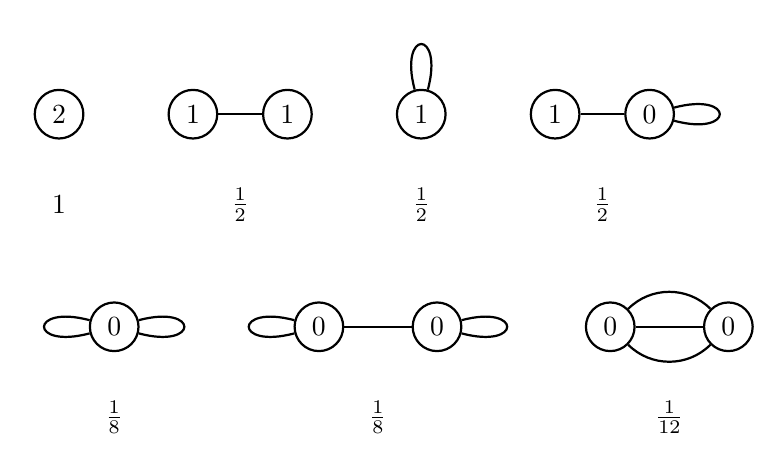
\begin{tikzpicture}[scale=1,transform shape,every loop/.style={min distance=8mm,looseness=10}]
        \node[circle,draw=black,thick] (a) at (0,0) {$2$};
        \node at (0,-1.15) {$1$};

        \node[circle,draw=black,thick] (b1) at (1.7,0) {$1$};
        \node[circle,draw=black,thick] (b2) at (2.9,0) {$1$};
        \draw[thick] (b1) -- (b2);
        \node at (2.3,-1.15) {$\frac{1}{2}$};

        \node[circle,draw=black,thick] (c) at (4.6,0) {$1$};
        \draw[thick] (c) edge[loop above] (c);
        \node at (4.6,-1.15) {$\frac{1}{2}$};

        \node[circle,draw=black,thick] (d1) at (6.3,0) {$1$};
        \node[circle,draw=black,thick] (d2) at (7.5,0) {$0$};
        \draw[thick] (d1) -- (d2);
        \draw[thick] (d2) edge[loop right] (d2);
        \node at (6.9,-1.15) {$\frac{1}{2}$};

        \node[circle,draw=black,thick] (e) at (0.7,-2.7) {$0$};
        \draw[thick] (e) edge[loop left] (e);
        \draw[thick] (e) edge[loop right] (e);
        \node at (0.7,-3.85) {$\frac{1}{8}$};

        \node[circle,draw=black,thick] (f1) at (3.3,-2.7) {$0$};
        \node[circle,draw=black,thick] (f2) at (4.8,-2.7) {$0$};
        \draw[thick] (f1) -- (f2);
        \draw[thick] (f1) edge[loop left] (f1);
        \draw[thick] (f2) edge[loop right] (f2);
        \node at (4.05,-3.85) {$\frac{1}{8}$};

        \node[circle,draw=black,thick] (g1) at (7.0,-2.7) {$0$};
        \node[circle,draw=black,thick] (g2) at (8.5,-2.7) {$0$};
        \draw[thick] (g1) -- (g2);
        \draw[thick] (g1) to[bend left=45] (g2);
        \draw[thick] (g1) to[bend right=45] (g2);
        \node at (7.75,-3.85) {$\frac{1}{12}$};
    \end{tikzpicture}
    \caption{The seven stable graphs of genus two with no legs, labelled by the genera of the vertices and weighted by \(\frac{1}{\ab|\Aut\Gamma|}\). On the slides each vertex was drawn as its Riemann surface component.}%
    \label{fig:g2stable}
\end{figure}

\begin{rmk}
    These are dual graphs of stable curves and are not the graphs of~\Cref{fig:tropgraphs}, which are the rigid tropical types obtained by applying the tropical decomposition formula to the reduced theory of the log GLSM. The two lists of topologies happen to coincide here, but a vertex means something different in each. Here it is a component of the domain curve carrying a topological field theory tensor. There it is a level of a bipartite tropical curve carrying either a log or an \(\infty\)-vertex moduli problem.
\end{rmk}

For the formal route, we define the normalized potential intrinsically by
\[ P_2^{\lambda} \coloneqq \frac{Y}{I_0^2}F_2^{\lambda}, \qquad Y = L^5. \]
The complete graph sum lies in \(\Q[L,\mc{X}_1,\mc{X}_2,\mc{X}_3,\mc{Y}_1]\) and equals
\begin{align*}
    P_2^{\lambda} ={}& -\frac{1}{128}L^{12} - \frac{23}{960}L^8\mc{X}_1 - \frac{9}{640}L^8\mc{Y}_1 + \frac{109}{16000}L^7 \\
    &- \frac{3}{80}L^4\mc{X}_1^2 - \frac{19}{320}L^4\mc{X}_1\mc{Y}_1 - \frac{3}{80}L^4\mc{Y}_1^2 - \frac{1}{64}L^4\mc{X}_2 \\
    &+ \frac{19}{1920}L^3\mc{X}_1 - \frac{47}{48000}L^2 \\
    &- \frac{67}{1152}\mc{X}_1^3 - \frac{101}{1152}\mc{X}_1^2\mc{Y}_1 - \frac{5}{48}\mc{X}_1\mc{Y}_1^2 - \frac{1}{24}\mc{Y}_1^3 \\
    &- \frac{25}{288}\mc{X}_1\mc{X}_2 - \frac{1}{48}\mc{X}_2\mc{Y}_1 - \frac{19}{1152}\mc{X}_3.
\end{align*}
For clarity, this is the exact formal \(\lambda\)-twisted answer and is not \(F_2^{\mr{GW}}\). Note also that \(Y = L^5\) is the discriminant generator while \(\mc{Y}_1\) is a logarithmic derivative generator.

\subsection{Finite generation and the extended family}%
\label{sub:Finite generation and the extended family}

Recall the finitely generated ring \(\mc{R} = \Q[A,B_1,B_2,B_3,Y]\) from above, which we will grade by
\[ \deg A = \deg B_1 = 1, \qquad \deg B_2 = 2, \qquad \deg B_3 = 3, \qquad \deg Y = 0. \]
For \(\phi_k = I_{1,1}\cdots I_{k,k}H^k\) as before, set
\[ \wt{\Omega}^{\lambda}_{g,n} \coloneqq 5^{g-1}\ab(\frac{Y}{I_0^2})^{g-1}\Omega^{\lambda,\tau}_{g,n}. \]

\begin{thm}[Graded finite generation {\cite{GJRstructure}}]%
\label{thm:graded finite generation}
    We have
    \[ \wt{\Omega}^{\lambda}_{g,n}(\phi_{a_1}, \ldots, \phi_{a_n}) \in \bigoplus_{k \geq 0}\lambda^{5k}H^{2(3g-3+\sum_i a_i - 5k)}(\Mbar_{g,n},\Q)\otimes \mc{R}_{3g-3+\sum_i a_i}. \]
    Consequently, after assembling the bipartite rest graphs, the non-equivariant component of the extended family satisfies
    \[ P^{\mbf{C}}_{g,n} = 5^{1-g}\int_{\Mbar_{g,n}}\wt{\Omega}^{\mbf{C}}_{g,n}(\phi_1^{\otimes n}) = \ab( \frac{Y}{I_0^2})^{g-1}\int_{\Mbar_{g,n}}\Omega^{\mbf{C}}_{g,n}(\phi_1^{\otimes n}) \in \mc{R}_{3g-3+n}. \]
\end{thm}

In particular, at each fixed \((g,n)\) only finitely many graded monomials can appear, and only \(R\)-matrix orders up to \(3g-3+n\) can contribute.

We organize the extended theory using the bipartite graph sum
\[ \Omega^{\mbf{C},\lambda}_{g,n} = \sum_{\Gamma \text{ bipartite}} \frac{1}{\ab|\Aut\Gamma|}\prod_{v\in V_{\infty}(\Gamma)} C^{\infty}_{g_v,\mu_v}(\mbf{C};\vec{a}_v) \prod_{v \in V_0(\Gamma)}C^{\lambda}_{g_v,\vec{\delta}_v}(\vec{a}_v)\prod_{e \in E(\Gamma)}V_e, \]
where \(C^{\infty}\) is an effective or meromorphic vertex factor, \(C^{\lambda}\) is a formal zero-vertex correlator, the \(\mu_v\) and \(\vec{\delta}_v\) record incident degrees, and \(V_e\) is the edge factor. The limit \(\lambda \to 0\) is taken only after the complete graph sum. Setting \(\mbf{C}=0\) leaves the formal \(\lambda\)-twisted leading sector. Setting \(\mbf{C}=\mbf{C}^{\mr{eff}}\) and \(\lambda\to0\) recovers quintic Gromov-Witten theory. Differentiating a universal edge cuts it and produces the holomorphic anomaly equation, while leaving the effective vertices untouched.

To derive the holomorphic anomaly equation, write \(P^{\mbf{C}}_g \coloneqq P^{\mbf{C}}_{g,0}\) and introduce
\[ \mc{U} = B_1, \qquad \mc{V} = A + 2B_1, \qquad \mc{V}_2 = D\mc{U} + \mc{U}^2 - \mc{U}\mc{V}, \qquad \mc{V}_3 = (D+\mc{V})\mc{V}_2, \]
together with the two non-holomorphic directions
\[ \partial_1 = \partial_{\mc{U}}, \qquad \partial_0 = \partial_{\mc{V}} - \mc{U}\partial_{\mc{V}_2} - \mc{U}^2\partial_{\mc{V}_3}. \]

\begin{thm}[Holomorphic anomaly equation for the extended family {\cite{GJRstructure}}]
    We have
    \[ -\partial_0 P^{\mbf{C}}_g = \frac{1}{2}P^{\mbf{C}}_{g-1,2} + \frac{1}{2}\sum_{\substack{g_1+g_2=g\\g_1,g_2\geq1}}P^{\mbf{C}}_{g_1,1}P^{\mbf{C}}_{g_2,1}, \qquad -\partial_1 P^{\mbf{C}}_g = 0. \]
\end{thm}

We prove this by the cutting argument of~\Cref{sub:The holomorphic anomaly equation}, which works because the derivative of the \(R\)-matrix propagator is simply
\[ 5\mc{B}_{\partial_0} = \bar{\phi}_1 \otimes \bar{\phi}_1, \qquad 5\mc{B}_{\partial_1} = \bar{\phi}_0\otimes\bar{\phi}_2 + \bar{\phi}_2\otimes\bar{\phi}_0. \]
Derivatives of \(R^{-1}\) and of every edge remain inside the same graded ring, so cutting a differentiated edge closes up on lower-genus correlators in \(\mc{R}\). If we set \(\mbf{C}=0\), then we recover the same equations for the formal \(\lambda\)-twisted theory.

\subsection{Boundary conditions}%
\label{sub:Boundary conditions}

We will use two sources of conditions on the holomorphic ambiguity.

First, we use regularity at the orbifold or Landau-Ginzburg point \(q = \infty\), equivalently \(L \to 0\). For either the formal or an assembled extended potential \(F_g^{\star}\), set
\[ \mc{P}_g^{\mr{orb},\star} \coloneqq \ab(\frac{L}{I_0})^{2g-2}F_g^{\star} = \Phi_g^{\star}(\mc{X}_1,\mc{X}_2,\mc{X}_3,\mc{Y}_1,L^{-1},L^5). \]
\Cref{thm:graded finite generation} bounds the possible Laurent powers of \(L\), and the formal LG/CY identification says that after analytic continuation and identification of the normalized CY and LG bases, the same formal \(R\)-matrix polynomial describes both phases. Therefore
\[ \lim_{L\to0}\Phi_g^{\star}(\mc{X}_1,\mc{X}_2,\mc{X}_3,\mc{Y}_1,L^{-1},L^5) \text{ exists}, \]
and for \(f_g(Y) = \sum_{i=0}^{3g-3}a_{i,g}Y^i\) with \(Y = L^5\) the quintic bound is
\[ a_{i,g} = 0 \qquad \text{for } i \leq \ceil*{\frac{3(g-1)}{5}}. \]
Note that this is a statement about the assembled normalized graph contribution, and not about individual bare meromorphic or rubber vertex correlators.

Second, we study the conifold. Set
\[ q = 5^{-5}(1+t_c)^{-1}, \qquad T_c = \frac{I_1^{\mr{co}}(t_c)}{I_0^{\mr{co}}(t_c)}, \]
where \(I_0^{\mr{co}}, I_1^{\mr{co}}\) form a local conifold period pair normalized so that the vanishing flat coordinate satisfies \(T_c = 0\) at the conifold. Given a rational expression \(f\) in the finite generation data, we obtain its conifold value \(f^{\mr{co}}\) by substituting the Laurent expansions of all generators as series in \(T_c\). \Cref{thm:graded finite generation} gives the pole bound
\[ F_g^{\mbf{C},\mr{co}} = O\ab(T_c^{-(2g-2)}), \]
but what we need is the stronger \textit{gap} condition
\[ F_g^{\mr{co}} = \frac{c_g}{T_c^{2g-2}} + O(1), \]
namely that every intermediate negative power \(T_c^{-(2g-3)}, \ldots, T_c^{-1}\) vanishes. This is \(2g-2\) conditions and is not implied by finite generation.

\begin{conj}[Formal conifold gap]%
\label{conj:formal conifold gap}
    The formal \(\lambda\)-twisted potential has the universal leading term
    \[ F_g^{\lambda,\mr{co}} = \frac{(-1)^{g-1}B_{2g}}{2g(2g-2)T_c^{2g-2}} + O(1), \]
    where \(B_{2g}\) is a Bernoulli number.
\end{conj}

\begin{exm}
    In genus two the computed expansion begins
    \[ F_2^{\lambda,\mr{co}} = \frac{1}{240T_c^2} + \frac{31}{6000} - \frac{7169}{3600000}T_c + \frac{22951}{45000000}T_c^2 + O(T_c^3). \]
    This is the genus two gap, not merely the pole order bound.
\end{exm}

We must also consider the formal correlators with rational descendant insertions which occur in the rest graphs, namely
\[ C^{\lambda}_{g,\vec{\delta}}(\vec{a}) \coloneqq \ab< \frac{H^{3-a_1}}{-5H\ab(-\frac{5H}{\delta_1}-\psi_1)}, \ldots, \frac{H^{3-a_n}}{-5H\ab(-\frac{5H}{\delta_n}-\psi_n)}>^{\lambda}_{g,n} \]
with \(\delta_i \geq 1\) and \(a_i \in \ab\{0,1,2,3,4\}\).

\begin{conj}[Regularity with special insertions]%
\label{conj:special correlator regularity}
    We have \(\ab(C^{\lambda}_{g,\vec{\delta}}(\vec{a}))^{\mr{co}} = O(1)\).
\end{conj}

For fixed \(\vec{a}\) and \(\vec{\delta}\), individual terms in the \(\psi\)-expansion may have poles. Note that the assertion concerns the complete rational descendant insertion, whose negative powers cancel before the rest graph sum over \(\vec{a}\) is taken. It is a statement about these specific formal correlators rather than about every unassembled meromorphic correlator.

We can use~\Cref{conj:formal conifold gap,conj:special correlator regularity} to transfer the gap to quintic Gromov-Witten theory. A rest graph contribution has the shape
\[ \sum_{\vec{a}} \prod_{v \in V_{\infty}(\Gamma)}I_0^{2g_v-2+\ell(\mu_v)}C^{\infty}_{g_v,\mu_v}(\vec{a}_v)\prod_{v\in V_0(\Gamma)}C^{\lambda}_{g_v,\vec{\delta}_v}(\vec{a}_v), \]
and the \(C^{\infty}\) factors are finite polynomials in \(q\), so they are conifold regular. Then the formal leading gap together with regularity of the special correlators implies the gap for the extended family, and therefore for the quintic.

\begin{rmk}
    \Cref{conj:formal conifold gap,conj:special correlator regularity} are open in general, but have been verified for the quintic through \(g \leq 5\) by Guo-Janda-Ruan. The pole bound for the extended family is a theorem, and the gap follows from the two conjectures and is proved for \(g \leq 5\) by explicit computation. At the time of these lectures, the all-genus gap for quintic Gromov-Witten theory was therefore conditional on them and unconditional for \(g \leq 5\).\footnote{Subsequently, Chang--Guo--You--Zhang announced an all-genus proof of the conifold gap for quintic Gromov--Witten theory in~\cite{CGYZ2026}. The two formal-theory conjectures above are separate statements.}
\end{rmk}

Putting all of this together, we begin with the Picard-Fuchs data and compute the Givental \(R\)-matrix and the operator \(S_{\tau}(z)\). We then obtain the formal stable graphs and meromorphic rest graphs, use the holomorphic anomaly equation and finite generation, and finally impose the orbifold and conifold boundary conditions to determine \(F_g^{\mr{GW}}\).

